\scanpage{152}\mspage{26}
de la forme
\[
s'=\deleted{\unsure{s^{r^{\pi_0}}|s^{\pi_0}|2^{r^{\pi_0}}}}s^t,\ \text{avec}\quad t\ge\unsure{r|t}^{\pi_0},\ s\ge2
\tag*{\unsure{(3.13.)|(3.15.)}}
\]
(alors $s'\ge2^{(r^{\pi_0})}>r^{\pi_0}\ge r$), $\underline{\mathrm{Fl}}^{s'}M$ est stable sous le foncteur $p_1^{C_0}:\underline{\mathrm{Fl}}\,M\unsure{\mathrel{\text{---}}|\longrightarrow}\underline{\mathrm{Fl}}\,M$.

\unsure{En|Ên|Én} effet, si on applique la première partie du lemme au couple $(\unsure{r|s},s')$, on trouve que $X_1(f)$ est dans $M^{s''}$, avec $s''=s'^{(r^{\pi_0})}$. Mais
\[
s''=s'^{(r^{\pi_0})}=(s^t)^{(r^{\pi_0})}=s^{t\cdot r^{\pi_0}}
\begin{tikzpicture}[baseline=(eq.base)]
\node[inner sep=1pt] (eq) at (0,0) {$=$};
\draw (0,-0.22)--(0,-0.42);
\node[anchor=north,inner sep=1pt] at (0,-0.47) {$\substack{\text{car }t\ge r^{\pi_0}\\\text{donc }t r^{\pi_0}=t}$};
\end{tikzpicture}
s^{t\unsure{.}}=s'
\]
donc on voit que $f\in\mathrm{Fl}^{s'}$ implique $X_1(f)\in M^{s'}$, ou ce qui revient au même, $p_1(f)\in\mathrm{Fl}^{s'}$.

\uline{Corollaire} \unsure{Soient|Soit} $C_0,r,s'=s^t$ ($t\ge r^{\pi_0}$, \inserted{$s\ge2$}) comme dessus, et soit $\alpha$ un nombre ordinal \deleted{de}\inserted{tel} \deleted{cardinal} que
\[
\mathrm{card}\,\alpha\le s'=s^t.
\]
Alors $\underline{\mathrm{Fl}}^{s'}M$ est stable par le foncteur $p_\alpha=p_\alpha^{C_0}$.

On le voit aussitôt par récurrence transfinie, compte tenu du lemme 3.3, et de l'hyp. de stabilité 3.13.

Pour résumer

\uline{Théorème 2} Soit $M$ une catégorie stable par \inserted{\unsure{petites|petite}} $\underset{\longrightarrow}{\lim}$ filtrantes, et munie d'une filtration cardinale $(\mathrm{Filt}^\pi)_{\pi\ge\pi_0}$, telle que les $\mathrm{Filt}^\pi$ soient stables par $\underset{\unsure{\mathrel{\text{---}}|\longrightarrow}}{\lim}$ filtrantes de cardinal $\le\pi$ (pas \unsure{forcément} grandes \unsure{devt|devant} $\pi_0$), et par \inserted{les} sommes amalgamées simples qui existent dans $M$. On suppose que les éléments de $\mathrm{Filt}^{\pi_0}$ soient accessibles, et on désigne par $\pi_1$ le plus petit cardinal $\ge\pi_0$, tel que les objets de $\mathrm{Filt}^{\pi_0}$ soient $\pi_1$-accessibles. On \unsure{pose} \deleted{de plus}
% archive sheet number: 151
